% Options for packages loaded elsewhere
\PassOptionsToPackage{unicode}{hyperref}
\PassOptionsToPackage{hyphens}{url}
\PassOptionsToPackage{dvipsnames,svgnames*,x11names*}{xcolor}
%
\documentclass[
]{article}
\usepackage{lmodern}
\usepackage{amssymb,amsmath}
\usepackage{ifxetex,ifluatex}
\ifnum 0\ifxetex 1\fi\ifluatex 1\fi=0 % if pdftex
  \usepackage[T1]{fontenc}
  \usepackage[utf8]{inputenc}
  \usepackage{textcomp} % provide euro and other symbols
\else % if luatex or xetex
  \usepackage{unicode-math}
  \defaultfontfeatures{Scale=MatchLowercase}
  \defaultfontfeatures[\rmfamily]{Ligatures=TeX,Scale=1}
\fi
% Use upquote if available, for straight quotes in verbatim environments
\IfFileExists{upquote.sty}{\usepackage{upquote}}{}
\IfFileExists{microtype.sty}{% use microtype if available
  \usepackage[]{microtype}
  \UseMicrotypeSet[protrusion]{basicmath} % disable protrusion for tt fonts
}{}
\makeatletter
\@ifundefined{KOMAClassName}{% if non-KOMA class
  \IfFileExists{parskip.sty}{%
    \usepackage{parskip}
  }{% else
    \setlength{\parindent}{0pt}
    \setlength{\parskip}{6pt plus 2pt minus 1pt}}
}{% if KOMA class
  \KOMAoptions{parskip=half}}
\makeatother
\usepackage{xcolor}
\IfFileExists{xurl.sty}{\usepackage{xurl}}{} % add URL line breaks if available
\IfFileExists{bookmark.sty}{\usepackage{bookmark}}{\usepackage{hyperref}}
\hypersetup{
  pdftitle={Energy Insecurity and Redlined America},
  pdfauthor={A. Justin Kirkpatrick},
  colorlinks=true,
  linkcolor=blue,
  filecolor=Maroon,
  citecolor=blue,
  urlcolor=blue,
  pdfcreator={LaTeX via pandoc}}
\urlstyle{same} % disable monospaced font for URLs
\usepackage[margin=1in]{geometry}
\usepackage{longtable,booktabs}
% Correct order of tables after \paragraph or \subparagraph
\usepackage{etoolbox}
\makeatletter
\patchcmd\longtable{\par}{\if@noskipsec\mbox{}\fi\par}{}{}
\makeatother
% Allow footnotes in longtable head/foot
\IfFileExists{footnotehyper.sty}{\usepackage{footnotehyper}}{\usepackage{footnote}}
\makesavenoteenv{longtable}
\usepackage{graphicx,grffile}
\makeatletter
\def\maxwidth{\ifdim\Gin@nat@width>\linewidth\linewidth\else\Gin@nat@width\fi}
\def\maxheight{\ifdim\Gin@nat@height>\textheight\textheight\else\Gin@nat@height\fi}
\makeatother
% Scale images if necessary, so that they will not overflow the page
% margins by default, and it is still possible to overwrite the defaults
% using explicit options in \includegraphics[width, height, ...]{}
\setkeys{Gin}{width=\maxwidth,height=\maxheight,keepaspectratio}
% Set default figure placement to htbp
\makeatletter
\def\fps@figure{htbp}
\makeatother
\setlength{\emergencystretch}{3em} % prevent overfull lines
\providecommand{\tightlist}{%
  \setlength{\itemsep}{0pt}\setlength{\parskip}{0pt}}
\setcounter{secnumdepth}{5}
\usepackage{bbm}
\usepackage{threeparttable}
\usepackage{float}
\usepackage{booktabs}
\usepackage[labelfont={bf}]{caption}
\usepackage{longtable}
\usepackage{array}
\usepackage{multirow}
\usepackage{wrapfig}
\usepackage{colortbl}
\usepackage{pdflscape}
\usepackage{tabu}
\usepackage{threeparttablex}
\usepackage[normalem]{ulem}
\usepackage{makecell}
\usepackage{xcolor}

\title{Energy Insecurity and Redlined America}
\author{A. Justin Kirkpatrick}
\date{}

\begin{document}
\maketitle

\hypertarget{thanks-heartland-2017-brian-murray-and-nicinstitute}{%
\subsubsection{Thanks: Heartland 2017, Brian Murray and NicInstitute}\label{thanks-heartland-2017-brian-murray-and-nicinstitute}}

\hypertarget{introduction}{%
\section{Introduction}\label{introduction}}

Energy insecurity has become a growing issue amongst policymakers. The energy insecurity literature shows evidence that low-income households frequently face
excessive energy bills, despite their income limitations, that initially seem counter-intuitive
\citep{Drehobl2016, Hernandez2013, Hernandez2010}. Poliycmakers have expressed concern not just that low-income
households spend a larger share of income on energy services, a measure known as \emph{energy burden}, but that low-income households are
paying more to attain the \emph{same} level of energy services relative to other income groups. The notion
of this inequity in ``energy access'' - the ability to purchase energy services such as home heating or cooling - has
been the object of programs that aim to improve residential energy efficiency through retrofits (CITE),
or provide subsidies for newer, higher-efficiency appliances (CITE). As part of increasing concerns
about income inequality, energy burdens and energy access inequity have become notable issues. This paper
explores the role of historic housing discrimination known as ``redlining'' and its potential role
in exacerbating energy access issues.

That a high energy burden is common amongst low-income households is not surprising as energy burden is,
by definition, decreasing in income. In an analysis of US Census American Housing Survey data, \citet{Drehobl2016} find city-level median energy burdens
of up to 12\%, with a 75th percentile as high as 26\% in the least energy-efficient location, Memphis, TN.
The existence of retrofit programs and home heating assistance programs like LIHEAP show that policymakers view home heating as a necessity \citep{Stein2018b}. Evidence
shows that inadequate home heating can cause or worsen existing medical issues (CITE), and
can affect child development and achievement (Cook et al., 2008?). However, these programs can be
expensive, suffer from economic dead weight loss due to poor targeting (CITE), under-deliver
promised results (Fowlie et al.), can interact with environmental and environmental justice goals negatively by subsidizing consumption
of energy (Levinson?), and are econommic ``second best'' to programs that successfully target the
source of the burden directly.

A racial component exists even beyond income-based energy inequity. Even when controlling for poverty rates, \citet{Reames2016}
finds that minority-dominated census block-groups and those block-groups with
high measures of racial segregation also tend to have lower (worse) energy efficiency and
thus spend a greater total amount for the same level of energy services relative
to non-minority households. Similarly, \citet{Drehobl2016} use American Housing Survey data to show that African-American and Latino households
face higher median energy burdens, even conditional on income. hat is That is, even conditional on poverty or income, minority areas and households
have lower-efficiency housing stock relative to non-minority areas and households. Not only is energy insecurity an issue, but so too is this ``energy inequity'',
which I define as ``the disproportional incidence of energy insecurity in heavily-minority areas
relative to non-minority areas of similar income.''

This energy inequity is primarily attributable to the housing stock, which is less energy effcient in low income and minority neighborhoods. Previous work in this area has found negative correlations between energy efficiency and racial characteristics at the census block-group level (Reames, 2016b), and many have noted the disproportionate energy burden faced by low-income households. With tight budget constraints, low-income households are more likely to consume lower-priced housing. Naturally, lower priced housing stock will be deficient
in some areas -- maintenance may be less frequent or non-existent, structural problems may plague the home, and the home may have un-remediated lead paint or asbestos. Similarly,
it is more likely that the home is poorly insulated, has single-pane windows, and has dated, inefficient systems for heating and cooling. To the extent that these deficiencies are priced into the sale or rental price of the home and are known equally to all potential purchasers or renters, then they should affect the energy usage of all purchasers or renters with similar income equally. The racial disparities noted in Reames (2016b) are a particularly unexplained phenomena.

This brings about the questions central to this paper: First, is there evidence that racial differences in
energy access exist once income and wealth are accounted for? Second, what drives the wedge between the energy
efficiency of the housing stock available to (or chosen by) minorities and the energy efficiency of
the housing stock available to (or chosen by) non-minorities of similar economic status?

This paper posits a hypothesis for one potential cause of this wedge and why it persists over time.
I propose that institutional discrimination in the 1930s-1970s forced African-Americans and other minorities into segregated ``redlined'' communities and,
over this period, the housing stock in these communities, though similar at one point in time, developed differently
relative to the housing stock of non-redlined communities of similar socio-economic standing and demographic
composition. This historical discrimination has persistent long-term effects on housing choices and housing quality
that explains, at least in part, the energy inequity we observe today.

To this end, I explore the extent to which
minority households inside and near the historic ``redlined'' neighborhoods face energy inequity - that is,
the extent to which minority households pay a higher amount for the same
level of energy services such as home heating relative to non-minorities of similar socio-economic status, which I do by
examining data on home energy consumption, race, and income. This requires careful attention to the nature of energy
expenditures. High levels of energy expenditure may be a sign that a household values warm temperatures during Winter
months and chooses to spend a larger share of income on home heating. High levels of energy expenditure may also be the result
of households who choose a home with very low energy efficiency and who must spend a great
deal simply to keep the interior temperature at a low but livable temperature. In short, one can spend a lot of money
to heat to 75 degrees farenheit in an efficient home, and one can spend an identical amount of money heating to 60 degrees farenheit
in a very inefficient home. The two are observationally equivalent when examining only monthly bills and relative outside temperature.
I disentangle these two by leveraging data from the California Residential Appliance Saturation Survey (RASS) which includes the consumer's reported thermostat setpoint,
combined with a simple model of household energy consumption. The model allows me to separate unobserved characteristics of the household
from home heating efficiency, permitting unbiased estimation of a household's home heating response to cold-weather shocks. By focusing on
the energy consumption response after controlling for the household's thermostat setpoint, I am able to measure the home's energy
efficiency level, rather than the household's preference for indoor temperatures or direct constraints on budgets.

Using original maps from the Homeowners Loan Corporation (HOLC) which designated ``redlined'' areas along with ``yellow'', ``green'' and ``blue'' areas
in more than 170 cities in the US in 1933-39 (Figure \ref{fig:HOLC1}),
combined with RASS survey data from 2009, I test the hypothesis that areas designated Grade D (or ``red''), which were considered ``appropriate'' for minorities to purchase homes, have more frequent substandard heating systems and are more inefficient in heating, evidenced by higher cost responses to cold weather shocks after controlling
for thermostat setpoints. As noted by \citet{Fishback2020}, the HOLC maps did not randomly assign neighborhoods grades and therefore any current differences in
the simple mean of energy efficiency outcomes between areas of different grades should not be causally attributed to redlining policy. Specifically, areas of lower construction quality, lower rent, older and smaller homes, and areas with pre-existing minority populations in 1933-39 were more likely to be graded as ``red.'' To address
the potential for bias, I control for these observables by using original survey data recorded by HOLC surveyors in 1933-39 that established the
justification for grading. Notably, there is considerable overlap in rents, the presence of minority populations, income, and other observables between ``red'' and ``yellow''
HOLC grades, leaving specific designation by the surveyor to be nearly random. Conditional on these observables and assuming that
unobserved differences correlated with HOLC grade do not still apply in the current period, then
``red'' grades are as good as randomly assigned. I use this conditionally as-good-as-random assignment to estimate causal effects of HOLC ``redlining'' on current
energy inefficiency and energy inequity.

\begin{figure}

{\centering 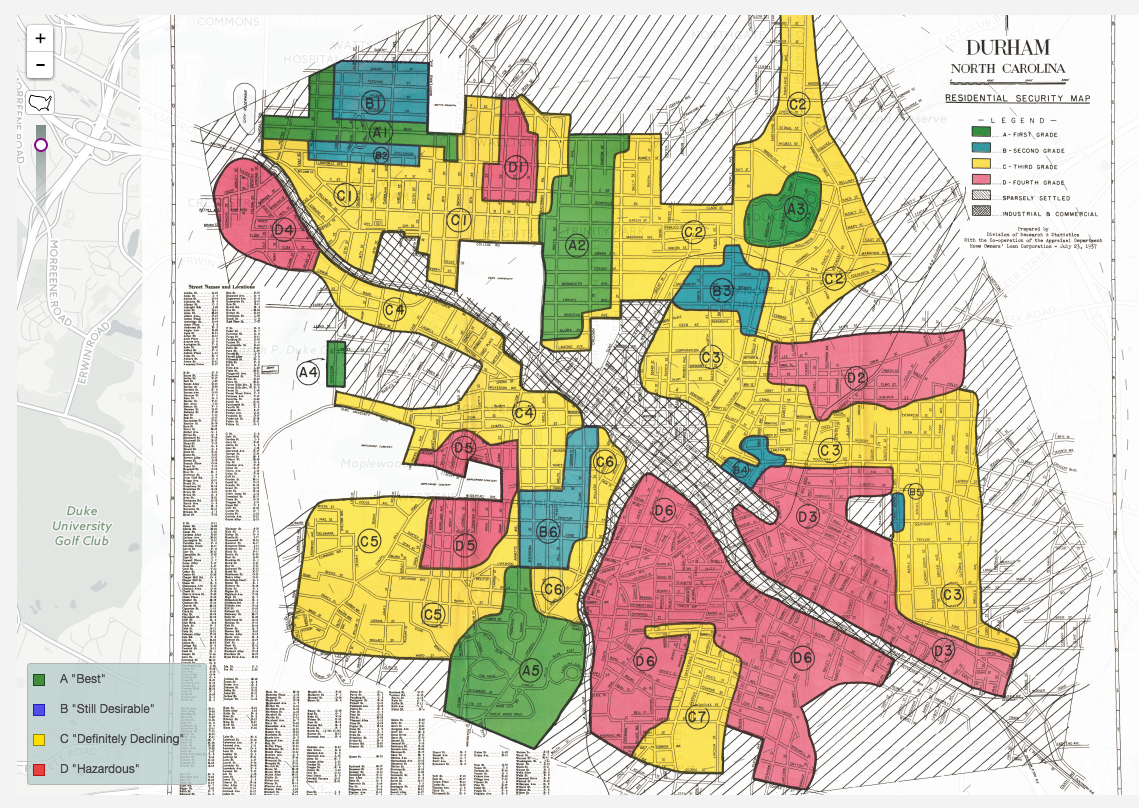
\includegraphics[width=0.9\linewidth]{D:/user/ajk41/Low Income Energy/Images/HOLC_example_1} 

}

\caption{Example of a HOLC map (1933) showing neighborhood designations in Durham, NC. Red areas were designated "appropriate" for lending to minorities, while other areas were not. \label{fig:HOLC1}}(\#fig:dispfig1)
\end{figure}

This paper does not address the dynamics of residential sorting between 1933 and the current period. While the practice of ``redlining'' came to a statutory end
with the Civil Rights Act of 1968, it was not until 1977's Community Reinvestment Act that lenders were required to detail the extent of their lending
in all areas in which they operated, including in heavily-minority ``redlined'' neighborhoods. \emph{De facto}, rather than \emph{de jure} housing discrimination continued
well beyond that date, and still continues today, albeit in different ways (see \citet{Christensen2020}). In a housing
market with no frictions and no discrimination, post-institutional redlining would have seen a re-sorting of households by preferences for housing stock. In
this perfect case, observed differences in energy inequity would be the result of households sorting in to inefficient units, and housing prices adjusting to
reflect the cost of heating. In effect, the most inefficient units would be rented by those who have little preference for warm tempertures. At the same time,
poverty is known to be cyclic, and low-income populations that rely heavily on family and community may have, in effect, high fixed costs of moving outside of a neighborhood. For young families especially, remaining close to (grand)parents may necessitate remaining in the same neighborhood for multiple generations. To the extent that a policy in place through 1977 ``fixed'' a family's location by precluding moves to other areas with better housing stock, the same families may face high costs of moving today resulting in a modern \emph{hysteresis} effect in redlined areas today. A full sorting model of residential choice is beyond this paper, though not infeasible under the right data circumstances.

This paper contributes to two separate literatures. The first literature
is the body of work that examines the role of historic discriminatory economic policies on
current outcomes. In this area, this paper is most similar to Aaronson and Mazumder (???), which specifically examines the effect of HOLC redlining on credit and home ownership, Aaronson and Mazumder use a boundary difference-in-differences to show that households located inside HOLC redlined areas had less access to credit and were less likely to own their home relative to similar households located just outside the boundary. That striking result motivates this paper -- one of the mechanisms by which energy inequity can manifest is through declining investment in available housing stock either by owner-occupants or by absentee landlords. Energy inequity is, at least in theory, a direct result of the effect shown by Aaronson and Mazumder.

The second literature
examines household electricity consumption responses to temperature or price shocks in the context of energy expenditures.
Largely motivated by the need to accurately predict future electricity consumption under future prices, demographics, or climate (Ang. and Auffhamer 2009),
these studies have examined the consumption response to varying temperature or prices. Few, however,
have incorporated a model of consumption that allows for endogenous preferences for thermostat setpoints. An exception is Brewer (2019), who estimates a ``bliss point''
in a structural model of joint residence and thermostat setpoint choice, though this paper examines moral hazard in landlord-paid heating.
The paper most similar to this is Doremus, Jacqz, and Johnston (2020), who examine household energy consumption expenditures in response to variation in temperature
by income. However, the authors similarly do not allow for endogenous thermostat setpoints that reflect unobserved tastes.

Section 2 defines energy inequity and introduces a simple model of home heating costs. It further shows how unobserved home efficiency characteristics,
which may vary between redlined and non-redlined neighborhoods when historic housing discrimination still impacts current energy burdens,\\
can be estimated from energy consmption data with a known thermostat setpoint. Section 3 introduces the data.
Section 4 discusses the estimation strategy. Section 5 presents results and Section 6 concludes.

Some citations: Aroonreuengsawat and Auffhammer: reponse to weather shocks, but does not endogenize the thermostat setpoint
Levinson 2013 (JEBO) on building codes: not using thermostats, just decomposing aggregate (state, region) decrease in PerCap energy by demos, moving, buildings, etc. Does use RECS, but only to get CA and NON-CA HDD responses (no thermostat)
Chong 2013: estimates response but no thermostat

\hypertarget{energy-inequity-and-housing-discrimination}{%
\section{Energy Inequity and Housing Discrimination}\label{energy-inequity-and-housing-discrimination}}

\hypertarget{the-energy-burden-and-energy-inequity}{%
\subsection{The Energy Burden and Energy Inequity}\label{the-energy-burden-and-energy-inequity}}

Energy burden is defined as the share of total household income spent on energy purchases not including transport. The low-income
energy burden is the noted phenomenon where low-income households have a disproportionate likelihood of having a high proportion
of household income devoted to energy purchases \cite{Byrne1986, Baxter1998}. In practice, energy burdens above 10\% are worrisome,
and many households have burdens of 20\% or more \cite{Baxter1998}. Middle and upper-income households tend to spend 5\% or less of
household income on energy services \cite{Hernandez2010}. High energy burden indicates an inability to afford
basic energy services (heating, refrigeration), particularly during periods of volatility in energy prices. High prices
or high volatility can lead to a ``heat or eat'' scenario \cite{HeatOrEat2003} where households must trade
off between heating and other necessities.

\hypertarget{conditional-on-income-problem-still-persists}{%
\paragraph{Conditional on income, problem still persists!}\label{conditional-on-income-problem-still-persists}}

Energy inequity can be defined as the gap between the cost to obtain a set level of energy services for a minority household
relative to a non-minority household of equal socioeconomic status and means. In earlier work, \cite{Reames2016} finds that minority-dominated census blocks and those with higher levels of racial segregation have higher heating costs per square foot, even conditional on income, and example of energy inequity. Energy services more broadly can be defined as
adequate lighting, heating, cooling, refrigeration, and sanitation. In this paper, I use home heating as the primary
energy serice discussed. The definition of energy inequity acknowledges that different households may have income-based differences in the selection of housing that lead to differences in the cost of energy services. Even beyond income-based constraints, heterogeneous preferences correlated
with race or ethnicity may still drive differences in total energy expenditures as households with preference for
warmer temperatures may forego other expenses in order to maintain a warmer home. By measuring the cost
to households to obtain a common level of energy services, rather than their oberved level, the measure accounts for these differences. Remaining, unexplained differences by race amongst households with similar socioeconomic statuses signify energy inequity.

\hypertarget{cite-severity-of-problem}{%
\paragraph{Cite severity of problem}\label{cite-severity-of-problem}}

Ramifications of insufficient heating with citations\ldots.

I focus on heating primarily because home heating represents the largest share of home energy consumption \cite{EIARECS2015} (2015 Residential Energy Consumption Survey: Energy Consumption and Expenditures Tables CE3.1). Furthermore, it is the energy expense that is most subject to heterogeneity across housing stock. The cost of heating is a function of three main inputs: the temperature setpoint relative to the outdoor temperature, the quality of the ``building envelope'' (e.g.~the presence of dual-pane windows or insulation), and the efficeincy of the heating source. The latter is affected by the type of fuel used. In general, substandard fuels like coal are highly inefficient. For fossil fueled heating systems like liquified petroleum gas (LP gas) or fuel oil, unit efficiency has improved over the last 30 years, and newer systems can be efficient. In the case of LP gas and fuel oil, however, cost tends to be higher \cite{EIARECS2015}, and systems require frequent delivery from distributers and storage on-site which tends to increase expense. Natural gas prices have declined since the early 2010's for most of the US, and efficiency of natural gas units has improved. Electric heat is not uncommon in much of the US, and the average expenditure for heating by electric is lower than fuel oil or LP gas, but higher than natural gas for most of the US \citep{EIARECS2015} (Table CE3.6). Electric furnaces and, more recenly, heat pumps have become more efficient. Overall, the cost per unit of energy for heat is higher for LP gas, fuel oil, and coal, lower for electricity and natural gas, and nearly always higher for older heating sources. This leads to two expectations: first, that households with no or substandard heating sources like coal will pay more to obtain the same level of heating than would households with natural gas or electric heat. Second, that households with older heating sources will pay more to obtain the same level of heating than would households with natural gas or electric heat.

\hypertarget{role-of-redlining-in-modern-energy-inequity}{%
\paragraph{Role of Redlining in Modern Energy Inequity}\label{role-of-redlining-in-modern-energy-inequity}}

Home efficiency, by definition, plays a large role in driving energy inequity, both through efficiency and age of heating equipment, and through building envelope integrity (drafts and leaks) and insulation. But what drives racial variation in home efficiency? Budget constraints may require a household to choose a less efficient house when on the purchase or rental market, but amongst households with the same socioeconomic status and budget constraint, the racial difference in efficiency implied by the energy inequity problem is not readily explained. This paper turns to a feature of US housing and credit policy known as ``redlining'' to provide a potential explanation for the racial energy inequity problem.

\hypertarget{redlining-was}{%
\paragraph{Redlining was\ldots{}}\label{redlining-was}}

Describe HOLC in depth here.

\hypertarget{causal-chain-is-really-long}{%
\paragraph{Causal chain is really long}\label{causal-chain-is-really-long}}

The relationship between current energy inequity and past redlining policies rests on three features of the housing market over the last 90 years:

First, the designation of ``hazardous'' lending areas (redlined areas) was a separating event that divided neighborhoods, including those with similar characteristics, along a policy-created line. A great deal of overlap in observable characteristics is observed between ``red'' and ``yellow'' areas, including comparable rent levels in 1933-1939, comparable racial compositions, and comparable quality of construction. Redlining specific neighborhoods provided a focus that organized the dynamics of housing and segregation. There is debate as to how formalized the HOLC maps were in bank lending decisions \citep{Hillier2003, Fishback2020}. Prior work has shown that redlined areas had historically higher interest rates for loans \citep{Hillier2003}, and this differential access to credit had widespread causal impacts on home ownership rates, home values, and subsequent disinvestment \citep{Aaronson2021}. Even absent a \emph{de jure} enforcement mechanism, the HOLC maps could have the same effect if the designations on the map lead to racial sorting of whites into non-red areas, and thus African-Americans into redlined areas. One testable implication of this ``separaing event'' is to test the rate of growth and in-migration of African-American households to ``red'' areas relative to those of observably similar ``yellow'' areas.

Second, the sorting of populations either through enforced lending practices or through informal \emph{de facto} segregation led to a divergence in the economic conditions, including credit access, within the redlined areas. As housing in ``red'' areas aged, stricter credit constraints and a lack of lending throughout the years resulted in a decline in the quality of homes and local disinvestment \citep{Aaronson2021}. This paper extends the findings of \citet{Aaronson2021} regarding credit access to the energy efficiency of the housing stock present in the redlined areas and tests for evidence of this divergence.

Third, even with the end of \emph{de jure} segregation across redlining and non-redlined areas, substantial costs to moving outside of a neighborhood still exist for those in a redlined area, imposing difficulty on those who seek more energy efficient housing. A number of sources of unobserved moving costs can by hypothesized. In particular, proximity to family who can assist with child-rearing is a particular (opportunity) cost imposed when moving to a new area. For families at or near the poverty line, grandparents or great-grandparents may provide childcare or meals for children when parents are working or otherwise unable to provide. Thus, the cost of moving to a different area with higher-quality and more efficient housing stock -- an area not negatively affected by years of disinvestment and ill repair -- may outweigh the potential benefits. Notably, in this situation, the prior effect of redlining policy maintains a \emph{hysteresis} effect on current energy burdens and energy inequity. In the absence of the HOLC maps and concordant redlining, this effect would not be present.

This paper does not fully model the causal chain of effect from 1933 to 2021. To address the first feature, I carefully test for observable differences between redlined and ``yellow'' HOLC grades. Results show that grade is influenced by the presence of African-Americans, but substantial overlap in characteristics between ``red'' and ``yellow'' neighborhoods exists. I leverage the overlap in observable characteristics that, I argue in subequent sections, provides as-good-as-random assignment of red grades. I also test for changes in rate of growth in ``red'' versus ``yellow'' neighborhoods of similar initial composition which provides support for the the first feature. The second feature is directly tested in this paper in the context of home heating fuel and home heating efficiency. Tests for consistency with the third feature are included, but no definite or causal claim is made or implied. It is likely that the data necessary to do so in the context of energy efficiency and the energy inequity problem does not exist -- electricity billing data at the address level is not available at large scale for any period prior to the 2000's.

\hypertarget{this-paper-here}{%
\subsection{This paper here\ldots{}}\label{this-paper-here}}

\hypertarget{explores-the-role-of-redlining-in-explaining-energy-burden}{%
\paragraph{Explores the role of redlining in explaining energy burden}\label{explores-the-role-of-redlining-in-explaining-energy-burden}}

By isolating the energy outcomes that can only be explained by redlining

\hypertarget{plausibly-exogenous-variation}{%
\paragraph{Plausibly exogenous variation}\label{plausibly-exogenous-variation}}

Conditional on similar (but not red-lined) nearby neighborhoods. Observables.

\hypertarget{extracted-1930s-data-to-understand-redlining}{%
\paragraph{Extracted 1930's data to understand redlining}\label{extracted-1930s-data-to-understand-redlining}}

Survey data created by federal HOLC employees in 1936-1939 provides neighborhood-specific data on observable characteristics that can be used to identify the effects of redlining. The designation of red- yellow-lined areas (as well as green and blue) aggregate away important variation between each grading. Not all redlined areas are identical, nor are all yellow areas. Survey data recorded as part of redline designation process provides important, but largely unusued, sources of variation. Within-grade variation in housing is common with reported average rents, median income, repair status of sing, share of housing developed, and construction type. Prior to being redlined, areas with high percentages of low-income or minority populations were more likely to have lower rents and lower housing lity. Frequently, the reason for a low-income or minority area's location was associated with the quality of the geography or proximity to natural features - low-lying areas that frequently flooded or as too steep for conventional building were generally populated by lower-income individuals. These same features also foment low investment in housing stock, and can explain current inefficiencies in sing regardless of the HOLC grade. With HOLC survey data in hand, I can control for these features and separate out the effect of HOLC redlining from the determinants of HOLC grading.

\hypertarget{identification-key-there-are-neighborhoods-with-identical-economics-and-racial-composition-where-some-surveyors-designated-them-red-and-some-designated-yellow.}{%
\paragraph{Identification key: there are neighborhoods with identical economics and racial composition where some surveyors designated them red and some designated yellow.}\label{identification-key-there-are-neighborhoods-with-identical-economics-and-racial-composition-where-some-surveyors-designated-them-red-and-some-designated-yellow.}}

\hypertarget{poor-whites-vs.-poor-blacks}{%
\paragraph{Poor whites vs.~poor blacks}\label{poor-whites-vs.-poor-blacks}}

\hypertarget{historic-data-merged-to-block-groups-to-leverage-modern-outcomes}{%
\paragraph{Historic data merged to block groups to leverage modern outcomes}\label{historic-data-merged-to-block-groups-to-leverage-modern-outcomes}}

\hypertarget{homeowners-loan-corporation-holc-grades}{%
\subsubsection{Homeowners Loan Corporation (HOLC) Grades}\label{homeowners-loan-corporation-holc-grades}}

The Homeowners Loan Corporation maps were generated by federal surveyors who were comissioned as part of a New Deal-era home mortgage refinancing and underwriting program intended to aid the residential real estate market during the Great Depression. The federal government, aiming to underwrite thousands of distressed mortgages thought partnerships with a new federal lending source and local banks, used the collected data to determine the risk of underwriting at a neighborhood level. Because of the need for fine spatial granularity, the spatial extent of the average ``neighborhood'' is around 1.1 square kilometers and contains around 15-50 residential blocks. Commercial and industrial areas and corridors are excluded. Data was collected approximately 1933-1939.

The surveyors mapped neighborhoods and collected data pertaining to their designation. Each neighborhood was designated in one of four ways:

\begin{itemize}
\item[A] "Best (Lending Area)" (Green)
\item[B] "Still Desirable" (Blue)
\item[C] "Definitely Declining" (Yellow)
\item[D] "Hazardous" (Red)
\end{itemize}

Designations were not necessarily fixed by any particular characteristic and no national standard appears to exist. While popular culture thinks of ``redlining'' as specifically racial, grading was influenced by the presence of African-American families, but was not purely derived from this information. The primary data collected on the survey is the racial composition of the neighborhood, the presence of ``subversive minorities,'' the African-American share\footnote{The surveyors do not use the term African-American} of the population, the type and condition of construction, rent and sale prices for the survey year, the professions of the residents, and the presence of ``relief'' families. Professions are noted in the surveys primarily because the location of residence within a city was largely determined by employment location and wage/job. Near a factory, one would often see a neighborhood for ``manual laborers'', another for management, and another for clerks and office-workers. When designating neighborhood grades, individual surveyors relied on relative populations and local context in setting grades rather than a national standard. This results in overlap in grading that can be leveraged to identify effects of interest. For instance, in downtown Detroit, there are neighborhoods where areas with 0\% African-American populations receive ``red'' grades (see: D37) yet adjacent neighborhoods with 20\% African-American populations receive ``yellow'' grades (see: C50).

To assess current energy outcomes, I merge original HOLC neighborhoods to modern census block groups, extracting ACS and census indicators of high energy burden. Census block groups match the granularity HOLC neighborhoods reasonably well. However, boundaries do not tend to coincide exactly, requiring some aggregation. Once linked, I compare modern energy outcomes with HOLC grading, conditioning on ervable characteristics both in the 1930's (selection), and in the present. While an individual household-level analysis would provide the clearest evidence, household-level energy consumption data is ited for privacy reasons, especially at the spatial resolution of HOLC neighborhoods, which can have as few as 100 homes in them.

\hypertarget{empirical-strategy}{%
\section{Empirical Strategy}\label{empirical-strategy}}

\hypertarget{home-heating-fuel}{%
\subsection{Home heating fuel}\label{home-heating-fuel}}

To estimate the impact of redlining on current energy outcomes, I focus on two main measures: the share of homes within a census block-group that report substandard heating fuel of either \textit{coal} or \textit{none}, and the energy consumption response of households. I first examine the prevalance of substandard heating fuel. Households with substandard heating fuel face the highest cost for home heating. I estimate the following regression:

\begin{eqnarray}
PercentSubstandard_{b} = \beta_0 + \sum_{g=1}^4 \beta_{g}^{Grade} +  \beta \mathbf{X}_b + \beta_{county} County_b + \epsilon_{b} \label{mainSubtandard1}
\end{eqnarray}

\begin{table}

\caption{(\#tab:substandard-est-1)Share of Households with Substandard Fuel (Coal and None) by HOLC Grade\label{tab:substandardnarrow1}}
\centering
\resizebox{\linewidth}{!}{
\begin{tabular}[t]{lccccccccccc}
\toprule
  & Model 1 & Model 2 & Model 3 & Model 4 & Model 5 & Model 6 & Model 7 & Model 8 & Model 9 & Model 10 & Model 11\\
\midrule
as.factor(GRADE.max)D & 0.00269** & 0.00263** & 0.00313* & 0.00279** & 0.00273** & 0.00320* & 0.00201* & 0.00195* & 0.00195* & 0.00273* & 0.00276*\\
 & (0.00119) & (0.00119) & (0.00159) & (0.00122) & (0.00122) & (0.00164) & (0.00111) & (0.00112) & (0.00111) & (0.00160) & (0.00160)\\
as.factor(GRADE.max)B & -0.00010 & -0.00002 & -0.00026 & -0.00003 & 0.00007 & -0.00021 & 0.00027 & 0.00019 & 0.00036 & -0.00004 & -0.00007\\
 & (0.00073) & (0.00074) & (0.00104) & (0.00071) & (0.00073) & (0.00104) & (0.00072) & (0.00074) & (0.00074) & (0.00101) & (0.00105)\\
as.factor(GRADE.max)A & 0.00017 & -0.00007 & -0.00213 & 0.00034 & 0.00010 & -0.00182 & 0.00074 & 0.00058 & 0.00049 & -0.00160 & -0.00157\\
 & (0.00188) & (0.00189) & (0.00266) & (0.00191) & (0.00192) & (0.00272) & (0.00191) & (0.00198) & (0.00194) & (0.00273) & (0.00283)\\
MedIncome2018 & -0.00011*** & -0.00011*** & -0.00010*** & -0.00012*** & -0.00012*** & -0.00012*** & -0.00012*** & -0.00011*** & -0.00012*** & -0.00012*** & -0.00012***\\
 & (0.00003) & (0.00002) & (0.00002) & (0.00002) & (0.00002) & (0.00002) & (0.00002) & (0.00002) & (0.00002) & (0.00002) & (0.00002)\\
MedIncome1936 & 0.00015*** & 0.00005 & 0.00023*** & 0.00016*** & 0.00005 & 0.00025*** & 0.00016*** & 0.00016*** & 0.00005 & 0.00025*** & 0.00025***\\
 & (0.00003) & (0.00011) & (0.00006) & (0.00004) & (0.00011) & (0.00006) & (0.00004) & (0.00004) & (0.00011) & (0.00007) & (0.00007)\\
Rent3739\_Mean & 0.00004** & 0.00004** & 0.00002 & 0.00004** & 0.00004** & 0.00002 & 0.00004** & 0.00004** & 0.00004** & 0.00002 & 0.00002\\
 & (0.00002) & (0.00002) & (0.00002) & (0.00002) & (0.00002) & (0.00002) & (0.00002) & (0.00002) & (0.00002) & (0.00002) & (0.00002)\\
MedIncome2018 × MedIncome1936 &  & 0.00000 &  &  & 0.00000 &  &  &  & 0.00000 &  & \\
 &  & (0.00000) &  &  & (0.00000) &  &  &  & (0.00000) &  & \\
\textcolor{red}{MaxRaceBlack} & \textcolor{red}{} & \textcolor{red}{} & \textcolor{red}{} & \textcolor{red}{-0.00201***} & \textcolor{red}{-0.00204***} & \textcolor{red}{-0.00234***} & \textcolor{red}{-0.00223***} & \textcolor{red}{-0.00244***} & \textcolor{red}{-0.00226***} & \textcolor{red}{-0.00246***} & \textcolor{red}{-0.00213**}\\
\textcolor{red}{} & \textcolor{red}{} & \textcolor{red}{} & \textcolor{red}{} & \textcolor{red}{(0.00075)} & \textcolor{red}{(0.00075)} & \textcolor{red}{(0.00071)} & \textcolor{red}{(0.00070)} & \textcolor{red}{(0.00072)} & \textcolor{red}{(0.00070)} & \textcolor{red}{(0.00071)} & \textcolor{red}{(0.00084)}\\
MaxRaceAsian &  &  &  & -0.00139* & -0.00143* & -0.00315*** & -0.00154** & -0.00201* & -0.00159** & -0.00321*** & -0.00301**\\
 &  &  &  & (0.00080) & (0.00082) & (0.00109) & (0.00076) & (0.00104) & (0.00076) & (0.00107) & (0.00126)\\
MaxRaceOtherRace &  &  &  & -0.00030 & -0.00035 & -0.00134 & -0.00027 & -0.00172 & -0.00033 & -0.00132 & -0.00227\\
 &  &  &  & (0.00181) & (0.00181) & (0.00172) & (0.00183) & (0.00132) & (0.00183) & (0.00173) & (0.00162)\\
NBlack\_YNTRUE &  &  &  &  &  &  & 0.00167 & 0.00088 & 0.00167 & 0.00092 & 0.00097\\
 &  &  &  &  &  &  & (0.00106) & (0.00081) & (0.00106) & (0.00074) & (0.00113)\\
NBlack\_YNTRUE × MaxRaceBlack &  &  &  &  &  &  &  & 0.00072 &  &  & -0.00083\\
 &  &  &  &  &  &  &  & (0.00141) &  &  & (0.00218)\\
NBlack\_YNTRUE × MaxRaceAsian &  &  &  &  &  &  &  & 0.00166 &  &  & -0.00103\\
 &  &  &  &  &  &  &  & (0.00319) &  &  & (0.00227)\\
NBlack\_YNTRUE × MaxRaceOtherRace &  &  &  &  &  &  &  & 0.00555 &  &  & 0.00411\\
 &  &  &  &  &  &  &  & (0.00458) &  &  & (0.00393)\\
\midrule
Num.Obs. & 6767 & 6767 & 4723 & 6767 & 6767 & 4723 & 6767 & 6767 & 6767 & 4723 & 4723\\
R2 & 0.131 & 0.131 & 0.117 & 0.132 & 0.132 & 0.119 & 0.133 & 0.134 & 0.133 & 0.119 & 0.119\\
R2 Adj. & 0.117 & 0.117 & 0.098 & 0.118 & 0.118 & 0.099 & 0.119 & 0.119 & 0.119 & 0.099 & 0.099\\
R2 Within & 0.024 & 0.024 & 0.024 & 0.026 & 0.026 & 0.026 & 0.026 & 0.027 & 0.026 & 0.026 & 0.027\\
R2 Pseudo &  &  &  &  &  &  &  &  &  &  & \\
AIC & -32741.4 & -32740.6 & -22720.7 & -32745.1 & -32744.5 & -22725.0 & -32748.5 & -32748.9 & -32747.9 & -22724.0 & -22721.3\\
BIC & -32018.5 & -32010.9 & -22074.6 & -32001.8 & -31994.3 & -22059.6 & -31998.4 & -31978.3 & -31990.9 & -22052.2 & -22030.0\\
Log.Lik. & 16476.715 & 16477.301 & 11460.327 & 16481.565 & 16482.241 & 11465.517 & 16484.266 & 16487.464 & 16484.933 & 11466.025 & 11467.630\\
FE: STCO & X & X & X & X & X & X & X & X & X & X & X\\
Std. errors & Clustered (STCO) & Clustered (STCO) & Clustered (STCO) & Clustered (STCO) & Clustered (STCO) & Clustered (STCO) & Clustered (STCO) & Clustered (STCO) & Clustered (STCO) & Clustered (STCO) & Clustered (STCO)\\
Block-Group HOLC Grade Threshold & 80\% & 80\% & 95\% & 80\% & 80\% & 95\% & 80\% & 80\% & 80\% & 95\% & 95\%\\
\bottomrule
\multicolumn{12}{l}{\textsuperscript{} * p $<$ 0.1, ** p $<$ 0.05, *** p $<$ 0.01}\\
\multicolumn{12}{l}{\textsuperscript{} Robust SE clustered by FIPS county}\\
\end{tabular}}
\end{table}

Where \textit{PercentSubstandard} is the census block-group share of households reporting substandard home heating fuel. \(\beta_{red}^{Grade}\) is the coefficient of interest which measures the difference in share of substandard heating fuel relative to the base category, which is ``yellow'' (Grade C), conditional on the controls. \(\mathbf{X}_b\) are controls for 2018 characteristics including median income and, in some specifications, current racial composition in the form of an indicator for the plurality race. \(\mathbf{X}_b\) also contains controls for characteristics from 1936-39 including median income, average rent, and a binary indicator for survey-reported presence of Black families. By including these historic characteristics, I control for the endogenous selection of some neighborhoods into the HOLC ``red'' grade. To the extent that surveyor-observable characteristics made a neighborhood more likely to be graded as ``red'', income and rents will control for these characteristics. Conditional on income, rent, and racial characteristics, ``red'' versus ``yellow'' HOLC grades were as good as randomly assigned. Implicit in this is the assumption that unobserved characteristics that led to a ``red'' grade no longer are present or influential in 2018 data. I test this below by residualizing the variation in HOLC grades and show (hopefully) that as-good-as-random assignment appears to hold -- no other observables explain assignment into ``red'' versus ``yellow'', indicating that surveyor effects are at play in designating grade.

HOLC grade D (red) areas with identical 1933-1939 characteristics to HOLC grade C (yellow) areas provide identification of the effect of redlining on current substandard household heating fuel provided historic observables sufficiently explain the designation of ``red'' versus ``yellow''. Combined with the assumption that redlined areas tend to have lower out-migration and tend to retain individuals within their neighborhood of birth\footnote{tested in Section \ref{assumptions} of this paper}, observing an increase in substandard heating attributed to redlining indicates that individuals whose parents or grandparents were limited, through policy, to residing within a redlined area are more likely to have a home with substandard heating fuel. Due to the cost of outmigration (e.g.~losing family support), individuals whose parents or grandparents resided in redlined areas face choice sets that are heavily weighted towards substandard heating fuel. Finding a significant difference across ``red'' and similar ``yellow'' neighborhoods in substandard heating fuel logically leads to a difference in the prevalence of substandard home heating fuel amongst blacks that persists once we condition on income, the leading indicator of energy inequity.

\hypertarget{household-response-to-heating-degree-days}{%
\subsubsection{Household response to heating degree days}\label{household-response-to-heating-degree-days}}

Equation \ref{mainSubstandard1} measures an outcome that proxies for overall heating system efficiency. However, it measures only one of the three determinants of a household's energy burden, which are (1) the efficiency of the heating source and the integrity of the building envelope; (2) the household's preferences for ambient indoor temperature; and (3) the household's income and budget constraints. Equation \ref{mainSubstandard1} captures only one portion of (1) is captured in the substandard heating fuel.

Observing disparities between the fuel source of redlined and non-redlined homes does not necessarily show that redlining is a driver of observed energy inequity. Some households may have low utility for home heating and thus prefer to live in homes with less expensive or older heating equipment, choosing a low thermostat setpoint. That is, for a household that prefers a low interior thermostat setting, there is little incentive to invest in (or rent a home with) a new, efficient heating unit. Aggregation to the block-group level can mask important heterogeneity in household energy consumption. I use household-level monthly consumption data geolocated to the zip-code level to identify HOLC-grade specific energy consumption responses to cooling and heating events.

Household preferences and the household budget constraint form an important set of conditions for interpreting the results of Equation \ref{mainSubstandard1}. A household may choose a home to rent or purchase that has substandard heating fuel if the household has a preference for lower-cost housing and little preference for warm ambient temperature. While households may have some preference for warmth, heterogeneity in preferences and in budget constraints suggests some households will select into these inefficiently-heated homes. Thus, I examine a second measure indicative of the energy burden -- the household response to heating degree days. As previously discussed, heating degree days are a measure of the difference between then outdoor daily high and a reference temperature. If the reference temperature is 64 degrees farenheit, and the daily high is 59 degrees farenheit, then the day is a 64-59 = 5 heating degree day. Formally, the equation is \(hdd_t = max\{0, \tau_t - T\}\) where \(\tau_t\) is the daily high, and \(T\) is the reference temperature. For the monthly measures used in this paper, heating degree days is formed by summing over all days in the month.

To measure household-level energy consumption response to weather-related shocks, I separately estimate a household response function of the form:

\begin{eqnarray}
energy^{j}_{ht} = \alpha_0 + \alpha_1^j hdd_{ht} + cdd_{ht} + \varepsilon_{ht} \label{mainResponse1}
\end{eqnarray}

Where \(energy^{j}_{ht}\) is the monthly total energy consumption for household \(h\) in month \(t\) for energy \(j\in \{gas,\quad electric\}\). Heating degree-days (\(hdd\)) and cooling degree-days (\(cdd\)) are specific to the household. Of interest is the \(\alpha_1\) term, the heating degree -day response \(hddr_h\) estimated for each household. Higher values of \(hddr_h\) indicate larger energy consumption responses. To test \(hddr\) across HOLC grades, I regress \(hddr_{h}\) on household-level and neighborhood characteristics.

\begin{eqnarray}
hddr^j_{h} = \delta_0 + \sum_{g=1}^4 \delta_{g}^{Grade} +  \delta \mathbf{X}_h + \varepsilon_{h} \label{mainResponse2}
\end{eqnarray}

Here, \(hddr^j_h\) is the household \(h\) response to \(hdd\) from Equation \ref{mainResponse1} for fuel \(j \in \{gas, \quad electric\}\). \(\delta_g^{Grade}\) is the estimate of the difference in \(hddr^j_h\) between HOLC grades using urban un-graded neighborhoods as the base level. \(\mathbf{X}_h\) includes the household's reported average annual income, home age, and dummy variables for each Climate Zone.

\begin{table}

\caption{(\#tab:RASS-1ex)Regression of heating-degree day gas consumption response on HOLC grade and income \label{tab:responsegas1}}
\centering
\begin{tabular}[t]{lcc}
\toprule
  & Model 1 & Model 2\\
\midrule
GRADE.maxD & 0.063** & 0.072**\\
 & (0.027) & (0.030)\\
GRADE.maxC & -0.227*** & -0.231***\\
 & (0.029) & (0.024)\\
avginc & 0.000 & 0.000\\
 & (0.000) & (0.000)\\
homeage &  & 0.001\\
 &  & (0.001)\\
kids &  & 0.004**\\
 &  & (0.002)\\
\midrule
Num.Obs. & 14822 & 14822\\
R2 & 0.107 & 0.117\\
R2 Adj. & 0.107 & 0.117\\
R2 Within & 0.004 & 0.015\\
R2 Pseudo &  & \\
AIC & 13135.9 & 12971.7\\
BIC & 13227.2 & 13078.2\\
Log.Lik. & -6555.968 & -6471.867\\
FE: CZT24 & X & X\\
Std. errors & Clustered (CZT24) & Clustered (CZT24)\\
\bottomrule
\multicolumn{3}{l}{\textsuperscript{} * p $<$ 0.1, ** p $<$ 0.05, *** p $<$ 0.01}\\
\multicolumn{3}{l}{\textsuperscript{} Using only households with gas as primary heating fuel}\\
\multicolumn{3}{l}{\textsuperscript{} Omitted grade is refactored to be "X"}\\
\end{tabular}
\end{table}

\begin{table}

\caption{(\#tab:RASS-2ex)Regression of heating-degree day electricity consumption response on HOLC grade and income\label{tab:responseelectric1}}
\centering
\begin{tabular}[t]{lcccc}
\toprule
  & Model 1 & Model 2 & Model 3 & Model 4\\
\midrule
as.factor(GRADE.max)D & 1.524 & 2.738 & 0.773 & 2.347\\
 & (2.189) & (3.038) & (2.129) & (2.868)\\
avginc & 0.000 & 0.000 & 0.000 & 0.000\\
 & (0.000) & (0.000) & (0.000) & (0.000)\\
cdd.e &  & 0.946*** &  & 0.937***\\
 &  & (0.232) &  & (0.217)\\
homeage &  &  & -0.052 & -0.016\\
 &  &  & (0.049) & (0.025)\\
kids &  &  & -0.118*** & -0.110***\\
 &  &  & (0.009) & (0.004)\\
\midrule
Num.Obs. & 2239 & 2239 & 2239 & 2239\\
R2 & 0.139 & 0.201 & 0.149 & 0.208\\
R2 Adj. & 0.135 & 0.197 & 0.144 & 0.203\\
R2 Within & 0.029 & 0.098 & 0.040 & 0.106\\
R2 Pseudo &  &  &  & \\
AIC & 17904.3 & 17740.2 & 17883.1 & 17724.2\\
BIC & 17967.2 & 17808.7 & 17957.4 & 17804.1\\
Log.Lik. & -8941.161 & -8858.087 & -8928.541 & -8848.078\\
FE: CZT24 & X & X & X & X\\
Std. errors & Clustered (CZT24) & Clustered (CZT24) & Clustered (CZT24) & Clustered (CZT24)\\
\bottomrule
\multicolumn{5}{l}{\textsuperscript{} * p $<$ 0.1, ** p $<$ 0.05, *** p $<$ 0.01}\\
\multicolumn{5}{l}{\textsuperscript{} Using only households with electricity as primary heating fuel}\\
\multicolumn{5}{l}{\textsuperscript{} Omitted grade is "X" for common comparison with gas as all "C" is lost in gas}\\
\end{tabular}
\end{table}

\hypertarget{a-model-of-heating-energy-consumption}{%
\subsubsection{A model of heating energy consumption}\label{a-model-of-heating-energy-consumption}}

Higher responses to heating degree days in HOLC ``red'' areas can be generated by two competing explanations. First, households in HOLC ``red'' areas may have less efficient homes and heating systems. When outside temperatures drop and \(hdd\) increases, a household with a poorly-sealed building envelope, drafty windows, and antiquated equipment will consume more energy to maintain the inside temperature relative to households with double-pane windows and newer heating systems maintaining the same temperature. A competing explanation is that HOLC ``red'' areas are more efficient, heating is less expensive on the margin, and households in these more efficient homes adjust by raising the thermostat setpoint. A home set at 72 degrees overnight may consume more energy during a cold spell than a home set at 55 degrees, even if it is more efficient. Looking only at household response is informative, but not necessarily unbiased.

To address this confounding, I construct a model of household energy consumption that leverages the household's response to a survey question on thermostat setpoint. Let heating energy consumed be determined by \(H(\kappa_i, \tau_{it}; \phi_i)\), where \(\kappa_i\) is the household's thermostat setpoint, \(\tau_{it}\) is the daily outside ambient temperature around household \(i\) on day \(t\), and \(\phi_i\) a parameter summarizing the envelope and appliance efficiency of household \(i\). Households with more efficient insulation, dual-pane windows, and higher energy star rated heating systems will have a lower value of \(\phi_i\). In a linear form, the cost of heating a home with setpoint \(\kappa_i\) in month \(m\) is:

\begin{eqnarray}
H = \phi_0 + \phi_i \sum_{d=1}^{D_m}max\{0, (\kappa_i - \tau_{id})\} \label{eq:hdd1}
\end{eqnarray}

The sum of ambient outdoor daily temperature deviations \(T_{id}\) from the thermostat setpoint \(\tau_i\) represents the sum of the temperature gradient between indoor and outdoor temperature. We do not observe the ambient outdoor temperature for each household, but do observe the monthly \(m\) heating degree days, which are \(\sum_{d=1}^{D_m}(\tau_{r(i)} - T_{id})\), where \(\tau_r\) is the heating degree days (HDD) reference temperature. The reference temperature varies by climate zone and is constant for each household across all time periods in the data. Rewriting \ref{eq:hdd1}:

\begin{eqnarray}
H &=& \phi_0 + \phi_i \sum_{d=1}^{D_m}\tau_i + \phi_i \sum_{d=1}^{D_m} \tau_r - \phi_i \sum_{d=1}^{D_m} T_{id} - \phi_i \sum_{d=1}^{D_m} \tau_r + \epsilon \nonumber \\
 &=& \phi_0 + \phi_i \sum_{d=1}^{D_m}(\tau_{r(i)} - T_{id}) + \phi_i \sum_{d=1}^{D_m}(\tau_i-\tau_{r(i)}) + \epsilon \nonumber \\
 &=& \phi_0 + \phi_i \sum_{d=1}^{D_m}(HDD_{id}) + \kappa_{i} + \epsilon \label{eq:hdd2}
\end{eqnarray}

OOPS, wait, HDD is max on 0. But I only use \textgreater0 months? The household thermostat setpoint \(\tau_i\) is time invariant. Thus, the household fixed effect absorbs the difference between the reference temperature and the thermostat
setpoint. If heating costs are not linear in deviations from \(\tau_{r(i)}\), \(\phi_i\) will capture both the household-specific efficiency, as well as the difference in
heating costs per HDD conditional on \(\tau_i\). For instance, if a household maintains a very high \(\tau_i>\tau_{r(i)}\) and faces convex costs in \(T_{i}\), \(\phi_i\) will
capture this difference. We estimate \(\phi_i\) over HOLC grades and household income. In our most flexible specification, we estimate a common \(\phi_i\) for each HOLC grade and for each value of \(\tau_i\) reported in the data. This is the household's energy consumption response to an increase in HDD conditional on the thermostat setpoint.

Conditioning on a specific overnight or daytime thermostat setting forecloses the possibility of bias due to household adjustment of thermostat settings or preferences for lower ambient temperatures. A household facing a budget constraint or with lower utility for ambient temperature may set the thermostat to a low setpoint. At this setpoint, the household will appear to spend less on energy than another household with a higher setpoint, which is observationally equivalent to a high-efficiency household. With this model, household consumption response functions for those that save on heating by setting the thermostat setpoint very low are identified by variation conditional on their setpoint. By allowing each setpoint bin
(\textless55, 55-60, 60-65, 65-70, 70-75, 75+) to have a separate estimate of response to heating degree days, I capture the effect of heating degree days separate from thermostat setpoint adjustments.

These estimates are the relevant estimates in examining the question of energy inequity. Instead of looking at total energy expenditures, I examine the cost of maintaining a consistent level of energy services (heat). It may remain that budget constraints cause some households to set their thermostats to a colder temperature than other households, and that energy inequity may still be a concern even if no difference in energy expenditure response to additional heating degree days is measured. I am conditioning out the long-run response (temperature setpoint) of the household to budget constraints. The remaining response identifies the cost to the household of maintaining a constant level of temperature.

Energy inequity is signified by a race-based difference in the response to heating degree days conditional on thermostat setpoint. To test for differences between redlined and non-redlined areas, I estimate separate coefficients for each HOLC grade in the data. I control for a variety of observed housing characteristics interacted with heating degree days onto control for other confounders that may determine a home's response to heating degree days separate from the HOLC grade. I account for Once properly conditioned, the difference between HOLC Grade D (red) and HOLC Grade C (yellow) housing can be estimated an

\[usage^g_i = \phi_0 + \phi_1 hdd_i + \phi_2 hdd_i*(grade_i=D) + \phi_3 averageincome_i*hdd_i + \phi_4 cdd^e_i*hdd_i + \sum_{s=1}^{S} hdd_i*\theta^s + \kappa_i + \varepsilon\]

Where \(usage^g_i\) is the monthly observed gas usage, \(hdd_i\) is the household's monthly heating degree days, \(s\in S\) are the temperature setpoint bins, and \(\kappa_i\) is a vector of household fixed effects.

\hypertarget{data}{%
\section{Data}\label{data}}

\hypertarget{homeowners-loan-corporation-holc-maps}{%
\subsection{Homeowners Loan Corporation (HOLC) Maps}\label{homeowners-loan-corporation-holc-maps}}

I obtain GIS shapefiles for the original HOLC grading maps for 202 cities over 38 states from the \href{https://dsl.richmond.edu/panorama/redlining/}{University of Richmond's \textit{Mapping Inequality} project} \citep{Nelson2021}. These maps have been digitized and georectified to align with modern street locations, allowing for a spatial merge to modern block groups, tracts, and zip codes. I spatially merge the HOLC neighborhoods to 2018 ACS Census blockgroups and 2018 Zip Code Tabulation Areas (ZCTAs). These are the finest spatial resolution available from the ACS that also includes data on primary home heating fuel and racial composition. I retrieve the Primary Home Heating Fuel Source variable from the 2018 ACS for each blockgroup and ZCTA that intersects any portion of a HOLC neighborhood.

Neither blockgroups nor ZCTAs align perfectly with HOLC neighborhoods. Blockgroups, which are drawn to follow municipal boundaries whenever possible, are the closest in scale and edges to the HOLC neighborhoods. However, even blockgroups are not perfectly aligned, and are certainly not 1:1. To obtain the HOLC neighborhood associated with a modern 2018 blockgroup, I tally the the spatial intersection shares for each blockgroup and designate each blockgroup by it's plurality HOLC grade. I include ``ungraded'' in this calculation to account for HOLC neighborhoods on the edge of city areas at the time of survey, and to account for ungraded commerical and industrial corridors that are incorporated into a modern blockgroup. I limit all samples only to those blockgroups where \(>80\%\) of the blockgroup, by area, overlaps with a single HOLC neighborhood grade. Because the blockgroups can still span multiple neighborhoods with the same HOLC grade, I aggregate characteristics of the HOLC neighborhood as a weighted mean where the weights are the spatial area shares exclusive of the ungraded areas.

I repeat the same process for ZCTAs, which are much larger aggregations. Because of the granularity of the HOLC maps and the larger extent of ZCTAs, far fewer ZCTAs have \(>80\%\) overlap with a single HOLC neighborhood grade, and thus sample sizes for ZCTA samples are sometimes too small for analysis.

To obtain the survey data from the University of Richmond's scanned and digitized surveyor sheets requires mapping the variables recorded across four or more formats of the survey questionnaire. Some questionnaires do not record, for instance, the nationalities of foreign families or the share of the population receiving relief. Some questionnaires report only the mean rent, while others report the rent range. Across the four separate questionnaire formats, important variables like percent African-American populations are listed in different areas of the report. To regularize across these various questionnaires, I map the consistent variables from each questionnaire and extract them into a regular table. I process the text to obtain numeric values for numeric variables, extracting the median of a range, and inferring the modal value of qualitative descriptions from those fields where a qualitative and quantitative value are given. For instance, the term ``few'' is often entered for percent African-American. In a handful of data fields for this question, the surveyor reports ``few - 2\%'' or ``few - 1\%''. For these qualitative answers, I use the modal associated value. ``Few'' becomes 1\%, ``nominal'' becomes 2\%, ``several'' and ``some'' become 3\%, ``scattered'' becomes 3.5\%,and ``small'' becomes 5\% based on the entries with both qualitative and quantitative reports.

In total, the data contains 44,357 blockgroups that intersect at least some of one or more HOLC neighborhoods. Of these, 25,827 intersect more than 80\% with a single HOLC grade, and 17,313 intersect more than 95\%. Table \ref{tab:datasummaryBG1} shows summary statistics for these blockgroups by sample.

\begin{table}

\caption{(\#tab:datasummary1)Summary statistics for blockgroups with 80 percent or more overlap (study) \label{tab:datasummaryBG1}}
\centering
\resizebox{\linewidth}{!}{
\begin{tabular}[t]{cllccc}
\toprule
HOLC Grade &   & Mean & Std. dev & Min Max & Missing\\
\midrule
D & Substandard Heating & 0.026 & 0.052 & [0.00, 0.47] & 15\\
 & Median Income 2018 & 51.805 & 34.703 & [2.50, 250.00] & 377\\
 & Median Income 1936 & 1.726 & 1.144 & [0.25, 25.00] & 2731\\
 & Share of largest overlap & 0.964 & 0.055 & [0.80, 1.00] & 0\\
 & Pct Black 1933 & 0.239 & 0.280 & [0.00, 1.00] & 2028\\
 & Blacks present & 0.506 & 0.500 & [0.00, 1.00] & 0\\
 & Mean Rent 1935 & 23.859 & 9.550 & [6.00, 75.00] & 3092\\
 & Mean Rent 37-39 & 25.460 & 8.746 & [6.00, 91.24] & 1840\\
C & Substandard Heating & 0.020 & 0.049 & [0.00, 0.50] & 7\\
 & Median Income 2018 & 54.874 & 28.845 & [5.51, 250.00] & 490\\
 & Median Income 1936 & 2.832 & 3.077 & [0.40, 53.00] & 5267\\
 & Share of largest overlap & 0.960 & 0.057 & [0.80, 1.00] & 0\\
 & Pct Black 1933 & 0.043 & 0.115 & [0.00, 1.00] & 4890\\
 & Blacks present & 0.184 & 0.387 & [0.00, 1.00] & 0\\
 & Mean Rent 1935 & 36.723 & 21.734 & [10.00, 420.00] & 5160\\
 & Mean Rent 37-39 & 39.157 & 20.837 & [10.00, 502.50] & 2614\\
B & Substandard Heating & 0.012 & 0.032 & [0.00, 0.36] & 5\\
 & Median Income 2018 & 70.029 & 41.556 & [4.02, 250.00] & 206\\
 & Median Income 1936 & 5.596 & 6.139 & [1.20, 51.00] & 2436\\
 & Share of largest overlap & 0.958 & 0.059 & [0.80, 1.00] & 0\\
 & Pct Black 1933 & 0.027 & 0.087 & [0.00, 0.80] & 2963\\
 & Blacks present & 0.071 & 0.257 & [0.00, 1.00] & 0\\
 & Mean Rent 1935 & 48.549 & 21.147 & [7.50, 434.14] & 2688\\
 & Mean Rent 37-39 & 58.103 & 38.758 & [0.00, 583.33] & 1877\\
A & Substandard Heating & 0.005 & 0.016 & [0.00, 0.16] & 1\\
 & Median Income 2018 & 110.159 & 62.291 & [7.22, 250.00] & 32\\
 & Median Income 1936 & 16.548 & 18.850 & [0.50, 100.00] & 721\\
 & Share of largest overlap & 0.952 & 0.061 & [0.80, 1.00] & 0\\
 & Pct Black 1933 & 0.010 & 0.097 & [0.00, 1.00] & 698\\
 & Blacks present & 0.028 & 0.166 & [0.00, 1.00] & 0\\
 & Mean Rent 1935 & 59.771 & 25.759 & [7.50, 174.60] & 766\\
 & Mean Rent 37-39 & 88.210 & 54.741 & [4.66, 524.68] & 537\\
X & Substandard Heating & 0.013 & 0.038 & [0.00, 1.00] & 196\\
 & Median Income 2018 & 66.546 & 40.952 & [2.50, 250.00] & 390\\
 & Median Income 1936 & 3.319 & 4.902 & [0.38, 66.79] & 3866\\
 & Share of largest overlap & 0.937 & 0.062 & [0.80, 1.00] & 0\\
 & Pct Black 1933 & 0.097 & 0.213 & [0.00, 1.00] & 3632\\
 & Blacks present & 0.172 & 0.378 & [0.00, 1.00] & 0\\
 & Mean Rent 1935 & 31.135 & 25.731 & [2.50, 450.00] & 3819\\
 & Mean Rent 37-39 & 34.939 & 27.740 & [0.00, 540.00] & 2508\\
All & Substandard Heating & 0.018 & 0.044 & [0.00, 1.00] & 224\\
 & Median Income 2018 & 61.763 & 39.062 & [2.50, 250.00] & 1495\\
 & Median Income 1936 & 3.511 & 5.575 & [0.25, 100.00] & 15021\\
 & Share of largest overlap & 0.955 & 0.059 & [0.80, 1.00] & 0\\
 & Pct Black 1933 & 0.106 & 0.212 & [0.00, 1.00] & 14211\\
 & Blacks present & 0.222 & 0.416 & [0.00, 1.00] & 0\\
 & Mean Rent 1935 & 35.092 & 22.564 & [2.50, 450.00] & 15525\\
 & Mean Rent 37-39 & 39.521 & 28.728 & [0.00, 583.33] & 9376\\
\bottomrule
\end{tabular}}
\end{table}

\hypertarget{census-blockgroups}{%
\subsection{Census blockgroups}\label{census-blockgroups}}

\hypertarget{substandard-heating-fuel-by-holc-grade}{%
\subsubsection{Substandard heating fuel by HOLC grade}\label{substandard-heating-fuel-by-holc-grade}}

\hypertarget{results}{%
\paragraph{Results}\label{results}}

Column 1 allows an additive effect for median income in 2018 and 1936 (reported from HOLC surveys), while 2-8 allow an interaction.

As expected, current median blockgroup income predicts a lower share of homes with substandard heating fuel across all models.
Median income in 1936 predicts \textbf{higher} prevalance of substandard heating in higher 1936 median income areas.

Columns 4-7 include controls for current racial composition.
These results consistently find that higher percentages of Blacks are associated with lower likelihood of substandard heating fuel. \textbf{EXPLAIN!!}

The coefficient on HOLC Grade D is positive and significant across almost all specifications, indicating that, conditional on a rich set of controls
including 1936 characteristics to control for selection on observables, areas that were graded ``D'' by the HOLC are more likely to have substandard
heating fuels in 2018 relative to those graded ``C''.

\hypertarget{results-1}{%
\paragraph{Results}\label{results-1}}

The same phenomenon is not observed when defining substandard heating as including LP gas and fuel oil. In many parts
of the country, LP gas and fuel oil are commonplace, and can be relatively efficient and desirable. It is not wholly
unexpected for this to be insignificant.

\hypertarget{household-level-energy-consumption-ca-rass}{%
\subsection{Household-level energy consumption (CA-RASS)}\label{household-level-energy-consumption-ca-rass}}

Household energy consumption data is retrieved from the California Residential Appliance Saturation Survey (RASS) for 2009 and (hopefully) 2019. The RASS
is commissioned by the California Public Utilities Commission and implemented by DNV GL Energy Insights. The survey contains information on household
energy consumption including home age, primary heating fuel source, and thermostat setpoint. The survey also includes the household's zip code,
household characteristics including income and number of children, and merges two years of billing information obtained direclty from the gas and electric
utilities serving the household. The survey sample consists of 25,721 households sampled from all over California.

We are interested in household's energy consumption response to increases in heating degree days. We focus on households that rely primarily on electric heating. For each household, we
estimate a consumption response function that summarizes the household's change in electricity consumption per change in monthly heating degree days.
This measure will be larger if a household consumes more energy when temperatures are lower, and smaller if a household consumes less energy when temperatures drop.
I allow this response to vary bsed on the HOLC grade that covers the plurality of the zip code in which the household lies. I use only those zip codes in which greater than 80\%
of the zip code is within one specific HOLC grade.

\emph{A priori}, it is not clear whether the interaction of heating degree days and HOLC-designated redlining should be positive or negative. If a household
prefers to remain warm and comfortable on a cold night, then expenditures will be higher when temperatures are lower. Similarly, if a household in a redlined area
maintains the same indoor temperature setpoint but has a home with lower energy ratings or is otherwise less efficient, then energy expenditures will be greater as well.
If expenditures are not greater, then it may be that the household trades off comfort by lowering the indoor temperature in order to keep expenditures low, or
it may be that the home is very efficient, and more energy is not needed to maintain a constant temperature. This ambiguity confounds interpretation of estimates.

Table (below) reports the results from a regression of the form:

\[hdd^e_h = \beta_0 + \sum 1(grade_h=g)\beta_g + \beta_{inc} avgincome_h + cdd^e_h + \gamma^{CZ} + \varepsilon\]

Where \(hdd^e\) is the electricity consumption response to one additional heating degree day for household \(h\) located in HOLC grade \(g\). \(cdd^e\) is the household's electricity consumption response
to an additional cooling degree day. Table (below that) shows results for \(hdd^g\). \(\gamma^{CZ}\) are climate-zone fixed effects.

Coefficient results in \ref{tab:responsegas1}, Model (1) indicate that households located inside the HOLC Grade D (red) areas
have significantly higher gas responses relative to those in HOLC ungraded areas within the urban boundary and relative
to those in HOLC Grade C. The omitted factor in \ref{tab:responsegas1} is ungraded so that results on Grade D can be
compared directly to \ref{tab:responseelectric1}, which has insufficient data to compare to Grade C.

Table \ref{tab:responseelectric1} shows significantly lower electricity responses.
In each case, only households that report primary heating fuel of gas (first table) and electricity (second table) are included.
The ambiguity in effect is clear in examining Table \ref{tab:responseelectric1}, which shows a significantly \emph{lower}
effect within the HOLC red (D) areas. In Grade D (red) areas, households using natural gas for their primary heating fuel
tend to have lower response to heating degree days relative to those in Grade C.

\begin{table}

\caption{(\#tab:RASS-1b)Regression of electricity consumption on heating degree days, interacted with HOLC grade and income, conditional on thermostat setpoint\label{tab:electricresponsethemset1}}
\centering
\resizebox{\linewidth}{!}{
\begin{tabular}[t]{lcccccccccc}
\toprule
  & Model 1 & Model 2 & Model 3 & Model 4 & Model 5 & Model 6 & Model 7 & Model 8 & Model 9 & Model 10\\
\midrule
hdd & 1.083*** & 1.068*** & 2.700*** & 2.644*** & 3.060*** & 2.632*** & 2.558*** & 3.615 & 0.769*** & 2.353***\\
 & (0.264) & (0.278) & (0.205) & (0.201) & (0.874) & (0.570) & (0.535) & (2.828) & (0.160) & (0.457)\\
hdd × GRADE.maxD & 3.729*** & 3.821*** & 2.917*** & 3.445*** & 4.569*** & 3.052*** & 2.980** & 4.615*** & 2.432*** & 2.701**\\
 & (0.407) & (0.407) & (0.728) & (0.614) & (0.697) & (1.153) & (1.189) & (1.300) & (0.873) & (1.205)\\
hdd × avginc & 0.000 & 0.000 & 0.000 & 0.000 & 0.000** & 0.000 & 0.000 & 0.000 & 0.000 & 0.000\\
 & (0.000) & (0.000) & (0.000) & (0.000) & (0.000) & (0.000) & (0.000) & (0.000) & (0.000) & (0.000)\\
hdd × cdd.e &  & -0.049 & -0.058* & -0.078* &  & -0.046 &  &  &  & \\
 &  & (0.036) & (0.031) & (0.044) &  & (0.097) &  &  &  & \\
hdd × NITESETOff &  &  & -1.348*** &  & 0.553 & 0.219 & 0.805 & -1.341 &  & 0.785\\
 &  &  & (0.454) &  & (0.758) & (1.269) & (1.403) & (1.393) &  & (0.901)\\
hdd × NITESET55-60 &  &  & -1.418* &  & -0.180 & 0.799 & 0.787 & -2.793 &  & 2.314\\
 &  &  & (0.769) &  & (0.611) & (1.851) & (2.147) & (4.820) &  & (2.156)\\
hdd × NITESET60-65 &  &  & -2.664*** &  & 0.643 & -0.245 & -0.167 & -1.363 &  & -0.218\\
 &  &  & (0.693) &  & (0.657) & (1.253) & (1.420) & (1.331) &  & (1.009)\\
hdd × NITESET65-70 &  &  & -0.604 &  & 1.187* & -0.088 & 0.476 & -0.861 &  & 1.432**\\
 &  &  & (0.536) &  & (0.656) & (1.519) & (1.364) & (1.134) &  & (0.575)\\
hdd × NITESET70-75 &  &  & -1.793*** &  & 2.068** & -1.828 & -1.876 &  &  & \\
 &  &  & (0.539) &  & (0.821) & (1.237) & (1.215) &  &  & \\
hdd × NITESETUnk &  &  & -1.921*** &  &  & 63.706 & 63.957** &  &  & \\
 &  &  & (0.163) &  &  & (42.665) & (27.479) &  &  & \\
hdd × DAYSETOff &  &  &  & -1.038** &  & -2.009* & -0.607 & 3.381*** &  & -1.973**\\
 &  &  &  & (0.508) &  & (1.205) & (1.307) & (1.048) &  & (0.828)\\
hdd × DAYSET55-60 &  &  &  & -2.035*** &  & -3.226 & -3.080 & 1.207 &  & -4.090*\\
 &  &  &  & (0.404) &  & (1.989) & (2.364) & (4.803) &  & (2.169)\\
hdd × DAYSET60-65 &  &  &  & -2.614*** &  & -3.106* & -2.564* & 4.964 &  & -2.813**\\
 &  &  &  & (0.891) &  & (1.778) & (1.480) & (3.407) &  & (1.106)\\
hdd × DAYSET65-70 &  &  &  & -1.333** &  & -0.795 & -1.122 & 1.779** &  & -2.303**\\
 &  &  &  & (0.573) &  & (1.426) & (1.341) & (0.731) &  & (1.017)\\
hdd × DAYSET70-75 &  &  &  & -1.421** &  & -1.556 & -1.805* & 2.222*** &  & -1.642***\\
 &  &  &  & (0.599) &  & (1.224) & (1.033) & (0.802) &  & (0.464)\\
hdd × DAYSETUnk &  &  &  & -1.978*** &  & -64.122*** & -64.032 & 1.923 &  & \\
 &  &  &  & (0.204) &  & (23.318) & (49.851) & (1.584) &  & \\
hdd × Rent3739\_Mean &  &  &  &  & -0.045** &  &  & -0.042 &  & \\
 &  &  &  &  & (0.021) &  &  & (0.064) &  & \\
hdd × DAYSETOff × as.factor(CZT24)3 &  &  &  &  &  &  &  &  & -0.360 & \\
 &  &  &  &  &  &  &  &  & (0.337) \vphantom{1} & \\
hdd × DAYSET55-60 × as.factor(CZT24)3 &  &  &  &  &  &  &  &  & -0.313** & \\
 &  &  &  &  &  &  &  &  & (0.129) & \\
hdd × DAYSET60-65 × as.factor(CZT24)3 &  &  &  &  &  &  &  &  & 0.629** & \\
 &  &  &  &  &  &  &  &  & (0.249) \vphantom{2} & \\
hdd × DAYSETUnk × as.factor(CZT24)3 &  &  &  &  &  &  &  &  & 0.126 & \\
 &  &  &  &  &  &  &  &  & (0.245) & \\
hdd × DAYSETOff × as.factor(CZT24)6 &  &  &  &  &  &  &  &  & 6.734*** & \\
 &  &  &  &  &  &  &  &  & (2.527) & \\
hdd × DAYSET55-60 × as.factor(CZT24)6 &  &  &  &  &  &  &  &  & 2.078 & \\
 &  &  &  &  &  &  &  &  & (4.860) & \\
hdd × DAYSET60-65 × as.factor(CZT24)6 &  &  &  &  &  &  &  &  & 8.594** & \\
 &  &  &  &  &  &  &  &  & (3.702) & \\
hdd × DAYSET65-70 × as.factor(CZT24)6 &  &  &  &  &  &  &  &  & 8.562** & \\
 &  &  &  &  &  &  &  &  & (3.914) & \\
hdd × DAYSET70-75 × as.factor(CZT24)6 &  &  &  &  &  &  &  &  & 14.078** & \\
 &  &  &  &  &  &  &  &  & (6.339) & \\
hdd × DAYSETUnk × as.factor(CZT24)6 &  &  &  &  &  &  &  &  & 0.000 & \\
 &  &  &  &  &  &  &  &  & (0.396) & \\
hdd × DAYSETOff × as.factor(CZT24)7 &  &  &  &  &  &  &  &  & 0.777 & \\
 &  &  &  &  &  &  &  &  & (1.000) & \\
hdd × DAYSET55-60 × as.factor(CZT24)7 &  &  &  &  &  &  &  &  & -0.328 & \\
 &  &  &  &  &  &  &  &  & (0.828) & \\
hdd × DAYSET70-75 × as.factor(CZT24)7 &  &  &  &  &  &  &  &  & 9.735*** & \\
 &  &  &  &  &  &  &  &  & (0.337) & \\
hdd × DAYSETUnk × as.factor(CZT24)7 &  &  &  &  &  &  &  &  & -0.676*** & \\
 &  &  &  &  &  &  &  &  & (0.140) & \\
hdd × DAYSETOff × as.factor(CZT24)8 &  &  &  &  &  &  &  &  & -1.270*** & \\
 &  &  &  &  &  &  &  &  & (0.198) & \\
hdd × DAYSET65-70 × as.factor(CZT24)8 &  &  &  &  &  &  &  &  & 1.679** & \\
 &  &  &  &  &  &  &  &  & (0.777) & \\
hdd × DAYSET70-75 × as.factor(CZT24)8 &  &  &  &  &  &  &  &  & 13.737*** & \\
 &  &  &  &  &  &  &  &  & (0.511) \vphantom{1} & \\
hdd × DAYSETOff × as.factor(CZT24)9 &  &  &  &  &  &  &  &  & 3.343*** & \\
 &  &  &  &  &  &  &  &  & (0.511) & \\
hdd × DAYSET60-65 × as.factor(CZT24)9 &  &  &  &  &  &  &  &  & -0.444* & \\
 &  &  &  &  &  &  &  &  & (0.249) \vphantom{1} & \\
hdd × DAYSET65-70 × as.factor(CZT24)9 &  &  &  &  &  &  &  &  & 0.500 & \\
 &  &  &  &  &  &  &  &  & (1.401) & \\
hdd × DAYSET70-75 × as.factor(CZT24)9 &  &  &  &  &  &  &  &  & 1.123** & \\
 &  &  &  &  &  &  &  &  & (0.515) & \\
hdd × DAYSETUnk × as.factor(CZT24)9 &  &  &  &  &  &  &  &  & 0.756*** & \\
 &  &  &  &  &  &  &  &  & (0.162) & \\
hdd × DAYSETOff × as.factor(CZT24)10 &  &  &  &  &  &  &  &  & 1.976*** & \\
 &  &  &  &  &  &  &  &  & (0.119) & \\
hdd × DAYSETUnk × as.factor(CZT24)10 &  &  &  &  &  &  &  &  & 1.041*** & \\
 &  &  &  &  &  &  &  &  & (0.145) & \\
hdd × DAYSETOff × as.factor(CZT24)12 &  &  &  &  &  &  &  &  & -15.282*** & \\
 &  &  &  &  &  &  &  &  & (0.249) & \\
hdd × DAYSET65-70 × as.factor(CZT24)12 &  &  &  &  &  &  &  &  & -2.562 & \\
 &  &  &  &  &  &  &  &  & (4.344) & \\
hdd × DAYSET>75 × as.factor(CZT24)13 &  &  &  &  &  &  &  &  & 1.811*** & \\
 &  &  &  &  &  &  &  &  & (0.206) & \\
hdd × DAYSETOff × as.factor(CZT24)13 &  &  &  &  &  &  &  &  & 0.125 & \\
 &  &  &  &  &  &  &  &  & (0.374) & \\
hdd × DAYSET60-65 × as.factor(CZT24)13 &  &  &  &  &  &  &  &  & -3.500*** & \\
 &  &  &  &  &  &  &  &  & (0.526) & \\
hdd × DAYSET70-75 × as.factor(CZT24)13 &  &  &  &  &  &  &  &  & -0.375 & \\
 &  &  &  &  &  &  &  &  & (0.597) & \\
hdd × as.factor(CZT24)6 × NITESETOff &  &  &  &  &  &  &  &  & -10.250*** & \\
 &  &  &  &  &  &  &  &  & (3.852) & \\
hdd × as.factor(CZT24)7 × NITESETOff &  &  &  &  &  &  &  &  & 0.941 & \\
 &  &  &  &  &  &  &  &  & (1.566) & \\
hdd × as.factor(CZT24)9 × NITESETOff &  &  &  &  &  &  &  &  & -0.779 & \\
 &  &  &  &  &  &  &  &  & (0.862) & \\
hdd × as.factor(CZT24)10 × NITESETOff &  &  &  &  &  &  &  &  & -2.041*** & \\
 &  &  &  &  &  &  &  &  & (0.000) & \\
hdd × as.factor(CZT24)6 × NITESET55-60 &  &  &  &  &  &  &  &  & -1.391 & \\
 &  &  &  &  &  &  &  &  & (5.999) & \\
hdd × as.factor(CZT24)7 × NITESET55-60 &  &  &  &  &  &  &  &  & 0.445 & \\
 &  &  &  &  &  &  &  &  & (0.565) & \\
hdd × as.factor(CZT24)10 × NITESET55-60 &  &  &  &  &  &  &  &  & 2.169*** & \\
 &  &  &  &  &  &  &  &  & (0.241) & \\
hdd × as.factor(CZT24)6 × NITESET60-65 &  &  &  &  &  &  &  &  & -7.875** & \\
 &  &  &  &  &  &  &  &  & (3.828) & \\
hdd × as.factor(CZT24)13 × NITESET60-65 &  &  &  &  &  &  &  &  & -0.125 & \\
 &  &  &  &  &  &  &  &  & (0.390) & \\
hdd × as.factor(CZT24)6 × NITESET65-70 &  &  &  &  &  &  &  &  & -7.812 & \\
 &  &  &  &  &  &  &  &  & (4.784) & \\
hdd × as.factor(CZT24)9 × NITESET65-70 &  &  &  &  &  &  &  &  & -0.514 & \\
 &  &  &  &  &  &  &  &  & (1.265) & \\
hdd × as.factor(CZT24)12 × NITESET65-70 &  &  &  &  &  &  &  &  & 0.938 & \\
 &  &  &  &  &  &  &  &  & (1.319) & \\
hdd × as.factor(CZT24)6 × NITESET70-75 &  &  &  &  &  &  &  &  & -7.656 & \\
 &  &  &  &  &  &  &  &  & (8.532) & \\
hdd × as.factor(CZT24)13 × NITESET70-75 &  &  &  &  &  &  &  &  & 0.375 & \\
 &  &  &  &  &  &  &  &  & (0.322) & \\
\midrule
Num.Obs. & 1150 & 476 & 476 & 476 & 593 & 476 & 1150 & 593 & 1150 & 855\\
R2 & 0.847 & 0.912 & 0.917 & 0.917 & 0.833 & 0.888 & 0.831 & 0.817 & 0.839 & 0.845\\
R2 Adj. & 0.825 & 0.890 & 0.894 & 0.893 & 0.804 & 0.855 & 0.805 & 0.783 & 0.809 & 0.820\\
R2 Within & 0.077 & 0.262 & 0.302 & 0.297 & 0.082 & 0.057 & -0.016 & -0.006 & 0.034 & 0.083\\
R2 Pseudo &  &  &  &  &  &  &  &  &  & \\
AIC & 15451.3 & 6323.9 & 6312.9 & 6316.5 & 8164.1 & 6470.1 & 15628.5 & 8255.6 & 15587.2 & 11693.9\\
BIC & 16163.0 & 6732.1 & 6746.1 & 6749.7 & 8558.7 & 6928.3 & 16400.7 & 8672.2 & 16521.0 & 12259.3\\
Log.Lik. & -7584.656 & -3063.967 & -3052.463 & -3054.233 & -3992.041 & -3125.057 & -7661.226 & -4032.781 & -7608.622 & -5727.942\\
FE: IDENT & X & X & X & X & X & X & X & X & X & X\\
Std. errors & Clustered (IDENT) & Clustered (IDENT) & Clustered (IDENT) & Clustered (IDENT) & Clustered (IDENT) & Clustered (IDENT) & Clustered (IDENT) & Clustered (IDENT) & Clustered (IDENT) & Clustered (IDENT)\\
\bottomrule
\multicolumn{11}{l}{\textsuperscript{} * p $<$ 0.1, ** p $<$ 0.05, *** p $<$ 0.01}\\
\multicolumn{11}{l}{\textsuperscript{} Using only households with electricity as primary heating fuel}\\
\multicolumn{11}{l}{\textsuperscript{} Omitted grade is "C"}\\
\end{tabular}}
\end{table}

Results have the expected sign - an increase in the heating degree days leads to an increase in electricity consumption across each of the specifications.
Households located inside a HOLC Grade D (red) area show around two to three times the consumption per hdd relative to the omitteed category, Grade C.
Unfortunately, too few households lie in HOLC areas with reported covariates necessary to control
for unobservables that may have affected the treatment (assignment to HOLC red) and the current outcome (home efficiency / gas consumption per hdd).\\
Column (3) through (7) control for the reported nighttime and daytime temperature setpoints. In both 3 and 4, the main effect remains (and increases in magnitude) - conditional on a target setpoint,
an increase in \(hdd\) leads to an increase in usage.
Although insignificant, the interaction for the two lowest bins, 55-60 and 60-65, is negative, indicating that an increase in \(hdd\) for households with very low overnight setpoints
leads to smaller increases in ELECTRICITY consumption relative to the omitted category, which is ``off/other''. As expected, households with very high overnight setpoints (\textgreater75) have very high
consumption responses to \(hdd\). In the last column, unknown thermostat setpoints are dropeed from the data. The effect of HOLC Grade D (red) persists.

Notably, households within the HOLC red (D) area continue to exhibit two to three times the consumption response relative to households in the omitted category, even accounting for
potentially heterogeneous preferences for overnight temperature setpoints. This indicates that households in HOLC red areas are not simply exhibiting greater preference
for overnight comfort, but rather face higher expenditures simply to maintain one constant temperature.

\begin{table}

\caption{(\#tab:RASS-1bGas)Regression of natural gas consumption on heating degree days, interacted with HOLC grade and income, conditional on thermostat setpoint\label{tab:gasresponsethemset1}}
\centering
\resizebox{\linewidth}{!}{
\begin{tabular}[t]{lcccccc}
\toprule
  & Model 1 & Model 2 & Model 3 & Model 4 & Model 5 & Model 6\\
\midrule
hdd & 0.283*** & 0.331*** & 0.236** & 0.304*** & 0.273*** & 0.274***\\
 & (0.071) & (0.083) & (0.092) & (0.102) & (0.088) & (0.100)\\
hdd × GRADE.maxlX & -0.055 & -0.038 & -0.056 & -0.100 & -0.109 & -0.093\\
 & (0.065) & (0.070) & (0.084) & (0.076) & (0.074) & (0.084)\\
hdd × avginc & 0.000 & 0.000 & 0.000 & 0.000 & 0.000 & 0.000\\
 & (0.000) & (0.000) & (0.000) & (0.000) & (0.000) & (0.000)\\
hdd × cdd.e &  & -0.006 & -0.006 & -0.005 &  & -0.005\\
 &  & (0.004) & (0.004) & (0.004) &  & (0.004)\\
hdd × NITESETOff &  &  & 0.093** &  & 0.049 & 0.101*\\
 &  &  & (0.046) &  & (0.046) & (0.056)\\
hdd × NITESET<55 &  &  & 0.076 &  & 0.100 & 0.123\\
 &  &  & (0.064) &  & (0.071) & (0.083)\\
hdd × NITESET55-60 &  &  & 0.226* &  & 0.168 & 0.231\\
 &  &  & (0.121) &  & (0.113) & (0.151)\\
hdd × NITESET60-65 &  &  & 0.185* &  & 0.111 & 0.152\\
 &  &  & (0.107) &  & (0.073) & (0.100)\\
hdd × NITESET65-70 &  &  & 0.119** &  & 0.063 & 0.102*\\
 &  &  & (0.052) &  & (0.049) & (0.061)\\
hdd × NITESET70-75 &  &  & 0.077 &  & 0.034 & 0.079\\
 &  &  & (0.062) &  & (0.052) & (0.085)\\
hdd × NITESETUnk &  &  & 0.066 &  &  & \\
 &  &  & (0.064) &  &  & \\
hdd × DAYSETOff &  &  &  & 0.030 & -0.027 & -0.041\\
 &  &  &  & (0.055) & (0.044) & (0.055)\\
hdd × DAYSET<55 &  &  &  & 0.016 & -0.101 & -0.108\\
 &  &  &  & (0.087) & (0.076) & (0.106)\\
hdd × DAYSET55-60 &  &  &  & 0.063 & -0.059 & -0.091\\
 &  &  &  & (0.059) & (0.070) & (0.093)\\
hdd × DAYSET60-65 &  &  &  & 0.190 & 0.040 & 0.061\\
 &  &  &  & (0.121) & (0.070) & (0.091)\\
hdd × DAYSET65-70 &  &  &  & 0.134* & 0.053 & 0.041\\
 &  &  &  & (0.078) & (0.051) & (0.063)\\
hdd × DAYSET70-75 &  &  &  & 0.110* & 0.043 & 0.020\\
 &  &  &  & (0.058) & (0.050) & (0.070)\\
hdd × DAYSETUnk &  &  &  & 0.037 & -0.036 & 0.064\\
 &  &  &  & (0.074) & (0.050) & (0.069)\\
\midrule
Num.Obs. & 3856 & 2177 & 2177 & 2177 & 3856 & 2177\\
R2 & 0.956 & 0.965 & 0.965 & 0.965 & 0.956 & 0.965\\
R2 Adj. & 0.946 & 0.956 & 0.956 & 0.956 & 0.946 & 0.956\\
R2 Within & 0.138 & 0.144 & 0.152 & 0.153 & 0.150 & 0.157\\
R2 Pseudo &  &  &  &  &  & \\
AIC & 42094.7 & 24577.6 & 24570.5 & 24567.8 & 42064.7 & 24569.0\\
BIC & 46462.3 & 27045.2 & 27077.9 & 27075.2 & 46513.7 & 27110.5\\
Log.Lik. & -20349.347 & -11854.806 & -11844.254 & -11842.904 & -20321.344 & -11837.512\\
FE: IDENT & X & X & X & X & X & X\\
Std. errors & Clustered (IDENT) & Clustered (IDENT) & Clustered (IDENT) & Clustered (IDENT) & Clustered (IDENT) & Clustered (IDENT)\\
\bottomrule
\multicolumn{7}{l}{\textsuperscript{} * p $<$ 0.1, ** p $<$ 0.05, *** p $<$ 0.01}\\
\multicolumn{7}{l}{\textsuperscript{} Using only households with natural gas as primary heating fuel}\\
\multicolumn{7}{l}{\textsuperscript{} Omitted grade is "C"}\\
\end{tabular}}
\end{table}

Unfortunately, we \textbf{lose all Grade D households in natural gas}.

\hypertarget{household-level-energy-by-ethnicity}{%
\paragraph{Household level energy by ethnicity}\label{household-level-energy-by-ethnicity}}

This section examines the coefficient of response across ethnicity (reported in RASS), as well as HOLC grade and thermostat set points.

\begin{table}

\caption{(\#tab:RASS-1c)Regression of electricity consumption on heating degree days, interacted with HOLC grade, ethnicity, and income, conditional on thermostat setpoint\label{tab:electricresponsethemset2}}
\centering
\resizebox{\linewidth}{!}{
\begin{tabular}[t]{lcccc}
\toprule
  & Model 1 & Model 2 & Model 3 & Model 4\\
\midrule
hdd & 1.601*** & 1.188*** & 1.585*** & 1.478***\\
 & (0.402) & (0.309) & (0.347) & (0.464)\\
hdd × GRADE.maxD & 1.764** & 1.120 & 1.770** & 1.351\\
 & (0.733) & (1.016) & (0.807) & (1.746)\\
hdd × ethnicityAsian and Pacific Islander & -0.674* & -0.467 & -0.948* & -0.782\\
 & (0.370) & (0.311) & (0.491) & (0.767)\\
hdd × ethnicityBlack & -0.869** & -0.460* & -0.982** & -0.708\\
 & (0.405) & (0.270) & (0.387) & (0.476)\\
hdd × ethnicityHispanic & -0.093 & 0.211 & -0.392 & -0.435\\
 & (0.546) & (0.511) & (0.583) & (0.943)\\
hdd × ethnicityOther & 2.066*** & 1.905*** & 1.755** & 1.895\\
 & (0.697) & (0.719) & (0.862) & (1.617)\\
hdd × ethnicityMixed & 2.119*** & 2.666*** & 1.848*** & 2.972\\
 & (0.383) & (0.662) & (0.566) & (2.169)\\
hdd × avginc1000 & -0.002 & -0.001 & -0.001 & -0.001\\
 & (0.003) & (0.003) & (0.003) & (0.004)\\
hdd × NITESETOff &  & 0.563 &  & 4.544***\\
 &  & (0.465) &  & (1.507)\\
hdd × NITESET55-60 &  & 0.256 &  & 1.259\\
 &  & (0.757) &  & (1.601)\\
hdd × NITESET60-65 &  & -0.978 &  & 1.794\\
 &  & (0.742) &  & (1.857)\\
hdd × NITESET65-70 &  & 1.182** &  & 2.471\\
 &  & (0.587) &  & (2.030)\\
hdd × NITESET70-75 &  & -0.160 &  & 2.687\\
 &  & (0.497) &  & (2.593)\\
hdd × DAYSETOff &  &  & 0.722 & -2.292\\
 &  &  & (0.533) & (1.414)\\
hdd × DAYSET55-60 &  &  & -0.697 & -2.657\\
 &  &  & (0.524) & (2.716)\\
hdd × DAYSET60-65 &  &  & -1.239 & -4.875***\\
 &  &  & (1.044) & (1.857)\\
hdd × DAYSET65-70 &  &  & 0.199 & -2.311\\
 &  &  & (0.675) & (1.437)\\
hdd × DAYSET70-75 &  &  & 0.248 & -3.262\\
 &  &  & (0.575) & (2.597)\\
\midrule
Num.Obs. & 1086 & 1086 & 1086 & 1086\\
R2 & 0.848 & 0.850 & 0.850 & 0.841\\
R2 Adj. & 0.826 & 0.827 & 0.827 & 0.817\\
R2 Within & 0.083 & 0.093 & 0.094 & 0.044\\
R2 Pseudo &  &  &  & \\
AIC & 14625.9 & 14624.4 & 14621.6 & 14707.4\\
BIC & 15314.6 & 15338.0 & 15335.2 & 15446.0\\
Log.Lik. & -7174.967 & -7169.180 & -7167.811 & -7205.697\\
FE: IDENT & X & X & X & X\\
Std. errors & Clustered (IDENT) & Clustered (IDENT) & Clustered (IDENT) & Clustered (IDENT)\\
\bottomrule
\multicolumn{5}{l}{\textsuperscript{} * p $<$ 0.1, ** p $<$ 0.05, *** p $<$ 0.01}\\
\multicolumn{5}{l}{\textsuperscript{} Using only households with electricity as primary heating fuel}\\
\multicolumn{5}{l}{\textsuperscript{} Omitted grade is "C"}\\
\end{tabular}}
\end{table}

Results surprisingly show that Black households with electricity as a primary heating fuel have lower responses to increases in heating degree days
relative to White households in two of the four specifications.
A similar effect holds for Hispanic households, though in no specifications are the results statistically significant
for Hispanic households. Conditioning on separate effects for nighttime and daytime thermostat setpoints reduces the magnitude of the
coefficient of response for households in HOLC grade red (D), but the point estimate is still positive.

\begin{table}

\caption{(\#tab:RASS-1cgas)Regression of gas consumption on heating degree days, interacted with HOLC grade, ethnicity, and income, conditional on thermostat setpoint\label{tab:gasresponsethemset2}}
\centering
\resizebox{\linewidth}{!}{
\begin{tabular}[t]{lcccc}
\toprule
  & Model 1 & Model 2 & Model 3 & Model 4\\
\midrule
hdd & 0.326*** & 0.307*** & 0.331*** & 0.308***\\
 & (0.082) & (0.088) & (0.090) & (0.088)\\
hdd × GRADE.maxlX & -0.093 & -0.110 & -0.122* & -0.118*\\
 & (0.072) & (0.073) & (0.071) & (0.071)\\
hdd × ethnicityNative American & -0.037 & -0.077 & -0.024 & -0.051\\
 & (0.053) & (0.074) & (0.054) & (0.063)\\
hdd × ethnicityAsian and Pacific Islander & -0.077*** & -0.066*** & -0.061** & -0.054**\\
 & (0.029) & (0.025) & (0.027) & (0.026)\\
hdd × ethnicityBlack & -0.069* & -0.056 & -0.054 & -0.038\\
 & (0.038) & (0.034) & (0.033) & (0.031)\\
hdd × ethnicityHispanic & -0.080*** & -0.063*** & -0.057** & -0.050**\\
 & (0.028) & (0.022) & (0.026) & (0.024)\\
hdd × ethnicityOther & 0.073 & 0.069 & 0.052 & 0.049\\
 & (0.056) & (0.048) & (0.063) & (0.058)\\
hdd × ethnicityMixed & -0.083** & -0.086* & -0.061* & -0.052\\
 & (0.039) & (0.052) & (0.033) & (0.036)\\
hdd × avginc1000 & 0.000 & 0.000 & 0.000 & 0.000\\
 & (0.000) & (0.000) & (0.000) & (0.000)\\
hdd × NITESETOff &  & 0.021 &  & 0.040\\
 &  & (0.035) &  & (0.046)\\
hdd × NITESET<55 &  & 0.007 &  & 0.068\\
 &  & (0.053) &  & (0.071)\\
hdd × NITESET55-60 &  & 0.112 &  & 0.145\\
 &  & (0.090) &  & (0.115)\\
hdd × NITESET60-65 &  & 0.043 &  & 0.054\\
 &  & (0.037) &  & (0.053)\\
hdd × NITESET65-70 &  & 0.052 &  & 0.045\\
 &  & (0.039) &  & (0.048)\\
hdd × NITESET70-75 &  & 0.028 &  & 0.032\\
 &  & (0.039) &  & (0.052)\\
hdd × NITESETUnk &  & -0.023 &  & -0.028\\
 &  & (0.047) &  & (0.052)\\
hdd × DAYSETOff &  &  & -0.014 & -0.035\\
 &  &  & (0.039) & (0.042)\\
hdd × DAYSET<55 &  &  & -0.063 & -0.131*\\
 &  &  & (0.061) & (0.072)\\
hdd × DAYSET55-60 &  &  & 0.013 & -0.062\\
 &  &  & (0.045) & (0.072)\\
hdd × DAYSET60-65 &  &  & 0.017 & -0.031\\
 &  &  & (0.039) & (0.052)\\
hdd × DAYSET65-70 &  &  & 0.069 & 0.038\\
 &  &  & (0.055) & (0.051)\\
hdd × DAYSET70-75 &  &  & 0.050 & 0.027\\
 &  &  & (0.041) & (0.048)\\
hdd × DAYSETUnk &  &  & -0.046 & \\
 &  &  & (0.051) & \\
\midrule
Num.Obs. & 3564 & 3564 & 3564 & 3564\\
R2 & 0.953 & 0.953 & 0.953 & 0.954\\
R2 Adj. & 0.943 & 0.943 & 0.943 & 0.943\\
R2 Within & 0.134 & 0.137 & 0.138 & 0.141\\
R2 Pseudo &  &  &  & \\
AIC & 38783.9 & 38786.0 & 38781.6 & 38782.2\\
BIC & 42806.2 & 42851.6 & 42847.2 & 42884.9\\
Log.Lik. & -18740.952 & -18735.022 & -18732.813 & -18727.119\\
FE: IDENT & X & X & X & X\\
Std. errors & Clustered (IDENT) & Clustered (IDENT) & Clustered (IDENT) & Clustered (IDENT)\\
\bottomrule
\multicolumn{5}{l}{\textsuperscript{} * p $<$ 0.1, ** p $<$ 0.05, *** p $<$ 0.01}\\
\multicolumn{5}{l}{\textsuperscript{} Using only households with natural gas as primary heating fuel}\\
\multicolumn{5}{l}{\textsuperscript{} Omitted grade is "C"}\\
\end{tabular}}
\end{table}

Table \ref{tab:gasresponsethemset2} shows an insufficient number of gas households in HOLC grade D (red) areas which precludes us from seeing the effect of HOLC red on response to heating degree days.
Results focused on ethnicity show that Hispanic households are less responsive to heating degree days conditional on daytime and nighttime
thermostat setpoints. A similar result for Black households is not significant.\cite{Reames2016} \cite{Baxter1998}

Should be a bib here
\printbibliography

\hypertarget{refs}{}

\hypertarget{appendix}{%
\section{Appendix}\label{appendix}}

\appendix

Apx text

\end{document}
